% Hetedik és nyolcadik előadás

\chapter{ARM processzorok}

Az ARM az Intel és az AMD mellett a harmadik nagy szereplő, a mobil világban egyeduralkodó.

\section{Terminológia}
Az ARM nem processzorgyártó cég, hanem CPU-kat, GPU-kat, NPU-kat és egyebeket fejlesztenek és a szellemi tulajdont értékesítik.
Ezzel szemben az Intel, AMD, Qualcomm stb. komplett processzorokat fejlesztenek és forgalmaznak, részben az ARM szellemi tulajdona alapján.
Ezért az ARM-re CPU - és nem processzor - fejlesztőként hivatkozunk.

\section{Áttekintés}
Az ARM egy brit félvezető fejlesztő cég (1983-ban alapították, Acorn RISC Machine, de 1990-től az Apple és a VLSI-vel közös projekttel Advanced RISC Machines), amit 2016-ban megvett egy japán bank, a Softbank.
2021-ben az Nvidia bejelntette, hogy megveszi az ARM-et, de ez még folyamatban van.
A cég alapvetően tervezéssel foglalkozik, kis áramfogyasztású processzor komponenseket és ezekhez kapcsolódó tervezési eszközöket fejleszt.
Ezek szellemi termékek, a bevételük ezeknek a licenszeléséből származik.

\subsection{Üzleti modell}
Az ARM a technológiát licenszeli a félvezető gyártó partnereinek, akik ezért licenszdíjat fizetnek.
A félvezető gyártó a legyártott processzorokat eladja az OEM gyártóknak (közben royalty-t fizetnek az ARM-nek), az OEM gyártók pedig végfelhasználói termékeket értékesítenek.
Az ARM figyelembe veszi a partnerek visszajelzéseit.
\begin{figure}[H]
    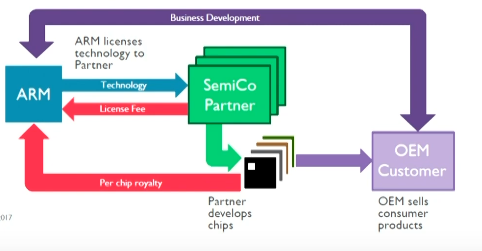
\includegraphics[width=0.7\textwidth]{armbm}
    \centering
    \caption{Az ARM üzleti modellje}
    \label{fig:armbm}
\end{figure}

\subsection{Licenszelés}
Az ARM két licenszet forgalmaz:
\begin{itemize}
    \item Cortex licensz: az ARM egy komplett mikroarchitektúrát értékesít, konfigurálható opciókkal
    \item Architektúra licensz: az ARM csak az ISA-t adja át a vevőnek, a vevő dolga megtervezni a saját mikroarchitektúráját (pl. Apple és Samsung)
\end{itemize}

\subsection{Az ARM dominanciájának okai}
Az ARM az x86-al szemben egy RISC architektúra, a RISC pedig Load/Store architektúra, tehát az operandusokat a regiszterekből olvassa be.
Az x86 viszont CISC és megenged operandus olvasást közvetlenül a memóriából.
Következmények:
\begin{itemize}
    \item a CISC utasítások nagyon hosszúak lehetnek a memória címzése miatt (base reg, offset, stb.)
    \item a RISC-eknél az utasításoknál elég a regisztereken címezni, a Load/Store-nál pedig a memóriát
    \item a CISC-ek utasításhossza változó, a RISC fix (általában 32 bit)
    \item a CISC-ek több áramot fogyasztanak, mivel az utasítás lehívás és a dekódolás komplexebb
\end{itemize}
A mobil világban nagyon fontos az alacsony fogyasztás, ezért a RISC alapú ARM architektúrák előnye.
Az ARM processzorok további fejlődésben vannak, újabban a szervereknél is kezdenek teret nyerni.
2020-ban, mikor az ARM-et megvette az Nvidia, az Nvidia CEO-ja kijelentette, hogy a desktopoknál is a legfontosabb architektúra az ARM lesz a jövőben.

\section{Az ARM ISA fejlődése}
 Az ARM (RISC) architektúra kezdetben kevés utasítást tartalmazott, de később az utasítások száma meghaladta az x86-ost is.
 Napjainkig 9 különböző ARM ISA verziót hoztak ki.
 Az első két verzióban még csak 26 bites címteret használt.
 Az ARMv3 volt az első olyan ISA verzió, ami már 32 bites címteret használt, ez tekinthető az ARM kiindulópontjának.
 Az ARM ISA jellemzői (korai változatok):
 \begin{itemize}
     \item 32 bites RISC architektúra
     \item 32 bites fixpontos vagy logikai adatokkal képes dolgozni
     \item 16 regisztert tartalmaz (13 általános + 3 dedikált)
 \end{itemize}
 A fejlődés négy fő irányban történt:
 \begin{itemize}
     \item számítási képességek növelése
     \item programkód méretének csökkentése
     \item bytekód végrehajtási sebesség növelése
     \item biztonság fokozása
 \end{itemize}
 A korai ARM rendszerek egyszerű, beágyazott alkalmazásokhoz készültek, ahol fontos volt a kód mérete és a bytekód végrehajtás sebessége is kritikus.
 A 2000-es években az ARM utat talált az alkalmazói processzorokba (mobilok), ahol sokkal általánosabb feladatokat kellett végrehajtania.
 Megjelent tehát a grafika és így a lebegőpontos számításokra való igény, megjelentek a SIMD utasítások is a számítási teljesítmény növelése érdekében.
 Fontossá vált a biztonság is.
 A v7-től kezdve a korábban fontosnak tartott szempontok értelmüket vesztették.

 \section{Számítási képességek fejlődése}
 Az ARMv3 egy egyszerű, alap architektúra, amit a fejlődés során kiterjesztettek.
 Egy utasításkészlet kiterjesztéséhez két dologra van szükség: egy regiszterkészlet definiálására és a regisztereken végrehajtható utasítások meghatározására.
 Az ARN fejlesztése három fő logikai lépésből állt:
 \begin{itemize}
     \item a műveletek kiterjesztése fixpontos SIMD utasításokkal (2002, ARMv6)
     \item másodlagos regiszterkészlet bevezetése skalár lebegőpontos, SIMD lebegőpontos és FX/FP lebegőpontos műveletekhez (2000, ARMv5)
     \item SVE regiszterkészlet (nagyon széles, 2KB) bevezetése, erre alapozva utasításkészlet kiegészítése (2016, ARMv8.2)
 \end{itemize}

 \subsection{Fixpontos SIMD kiterjesztés}
 Ezzel 32 bit szélesen lehetett végrehajtani 8 vagy 16 bites műveleteket (\ref{fig:fxsimd}).
 \begin{figure}[H]
    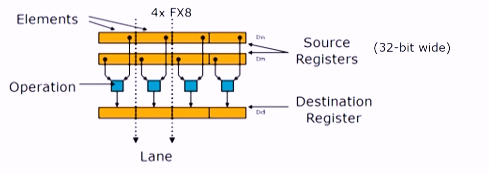
\includegraphics[width=0.7\textwidth]{fxsimd}
    \centering
    \caption{Fixpontos SIMD utasítások végrehajtása}
    \label{fig:fxsimd}
\end{figure}
Az ezzel elért teljesítmény növekedés csekély volt, ezért később kiterjesztették a NEON bővítménnyel.

Az ARMv8 ISA-jának két végrehajtási módja volt: 32 és 64 bites.
Az utóbbihoz kiterjesztették a regiszterkészletet, a 32 bites működés a kompatibilitást szolgálta.

\subsection{Lebegőpontos műveletvégzés}
A NEON kiterjesztés a multimédiás alkalmazások gyorsítását szolgálta.
Lehetővé tette, hogy 64 vagy 128 bites hosszú adatokon történjen a műveletvégzés.

\subsection{SVE regiszterkészletre alapuló SIMD kiterjesztések}
Az SVE-t (Scalable Vector Extension) 2016-ban mutatták be, az ARMv8.2 alapú ISA-ban.
Csak a 64 bites verzióban volt aktív.
Alapvető célja a HPC (High Performance Computing), tehát a tudományos jellegű, képfeldolgozó és média alkalmazások támogatása.
FX és FP műveleteket is támogat.
A regiszterkészlet nem volt rögzítve, hanem 128 bittől egészen 2 Kb hosszú regiszterek használhatók voltak, tehát többféle fixpontos és lebegőpontos adattípust is támogatott.
Ezeket hívták Z regisztereknek.

Legfontosabb jellemzője, hogy a programozásban nem kell figyelembe venni a hardveres regiszterek hosszát.
Így a programozóknak könnyebb kódot írnia, mivel eltérő végrehajtóegység méretű processzorokra ugyanazt a kódot tudja használni.
A megírt binárisok hordozhatóbbak és automatikus vektorizáció lehetséges a compilerekben.

A megvalósításhoz predikátum regisztereket vezettek be, amiket maszkokként használtak.
Ez megmutatja, hogy az adat melyik része aktív és melyik nem.
16 predikátum regiszter áll rendelkezésre.
A predikátum regisztereket a programkódban be kell állítani.

\subsection{SVE 2}
Az előző részben leírt SVE-t szinte nem használták.
Később bemutatták a továbbfejlesztett változatát, az SVE2-t (ARMv9, 2021).
A cél a HPC helyett egy széleskörű alkalmazás palettát támogatni és a NEON-t kiváltani.
\begin{figure}[H]
    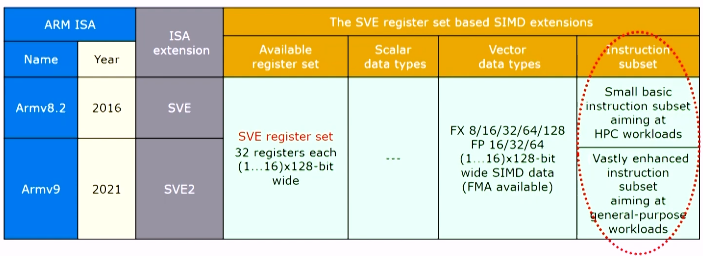
\includegraphics[width=0.8\textwidth]{sve}
    \centering
    \caption{Az SVE és SVE2 összehasonlítása}
    \label{fig:sve}
\end{figure}
Az SVE-t csak a Fujitsu A64FX processzora implementálta.
Ennek oka, hogy az eredeti SVE nagyrészt HPC feladatokra volt kitalálva, de a mobilok nem futtatnak ilyen alkalmazásokat.
Ezzel szemben az SVE2 elsősorban a szervereket célozza meg, ahol gyakoriak az ilyen feladatok.

\section{Az ARM CPU-k áttekintése}
Az ARM CPU-k csoportosítása:
\begin{itemize}
    \item Korai ARM CPU-k
    \begin{itemize}
        \item ARMv1 és v2 (1985-1990): 26 bites címbuszú rendszerek, nem tárgyaljuk őket. Pl.: ARM1-ARM3
        \item ARMv3-v6 (1991-2004): 32 bites rendszerek. Pl.: ARM6xx-ARM11xx
    \end{itemize}
    \item ARM Cortex CPU-k (ARMv7-v9): 2004-től, ma is ezek az uralkodók. 8.0-tól 64 bites
    \item ARM Neoverse CPU-k (ARMv9): 2021-től, szerverekhez készültek, teljesen új család
\end{itemize}

\subsection{Cortex CPU-k}
A Cortex CPU-k a jelenlegi mobil világ alapját alkotják.
2004-ben vezették be, elsőként a Cortex-M3 beágyazott processzorban.

\subsection{Cortex profilok}
A Cortex családot 3 különböző profilra osztották, felhasználás szerint:
\begin{itemize}
    \item Cortex-A: alkalmazások, a mai mobil processzorok alapja
    \item Cortex-R: kritikus, valós idejű rendszerek
    \item Cortex-M: mikrokontroller, nem annyira kritikus rendszerek
\end{itemize}

\subsubsection{Cortex-A profil}
Két utasításkészletet támogat: az A32-t és a T32-t.
A T32 egy 16 bites utasításokat tartalmazó részhalmaza az A32-nek.
Az ARMv8-A verzióval megjelent a 64 bites kiterjesztés, a korábbi 32 bites alkalmazásokkal kompatibilis módon.
A 32 bites alkalmazásokat AArch32 végrehajtási módban, A32 utasításkészlettel futtatja, a 64 biteseket pedig AArch64 módban, A64 utasításkészlettel.
Ezzel együtt az AArch64 módban megszüntették a Thumb 16 bites utasításkészlet támogatását.
Az ARMv9-el a 32 bites utasításokat sem támogatták tovább.

\subsubsection{Cortex-R profil}
Beágyazott rendszerekhez készült, szintén az A32 és T32 utasításkészleteket támogatja.

\subsubsection{Cortex-M profil}
Mélyen beágyazott rendszerekhez, mikrokontrollerekhez készült (pl. autóipar).
Ez csak a T32 16 bites utasításokat támogatja, hogy minél kisebb legyen a program.

\subsubsection{SecurCore profil}
2007-ben a családot kiegészítették a SecurCore profillal, smart card és egyéb biztonsági alkalmazásokra kifejlesztve.

A továbbiakban csak az A profilú processzorokkal foglalkozunk.

\section{A Cortex-A profilú CPU-k fejlődése (v7 és v8)}
2004-ben jelentek meg az első Cortex-A CPU-k, 2011-től támogatták a big.LITTLE felépítést (ARMv7-A ISA).
Ezt követték az ARMv8.0-A-t megvalósító, 64 bites CPU-k (2012-ben jelentették be).
A következő generáció (ARMv8.2-A, 2017) már támogatta DynamIQ magcsoportokat, ami a korábbi big.LITTLE magcsoportokat váltotta.
2021-ben megjelent az ARMv9-A, ahol jelentősen továbbfejlesztették a DynamIQ-t.

\subsection{Az ARMv7-8 CPU-k fejlődése}
Három teljesítmény osztályt határoztak meg:
\begin{itemize}
    \item nagy
    \item közepes
    \item alacsony teljesítményű, kis fogyasztású
\end{itemize}
Az eltérő teljesítményű rendszerekhez eltérő lapkaméretek is tartoznak.
A kis teljesítményű rendszerek viszonylag kis helyen megvalósíthatóak, míg a nagy teljesítményűekhez több helyre van szükség.

A Cortex-A CPU-k fejlődését négy szempont szerint vizsgáljuk:
\begin{itemize}
    \item szóhossz
    \item L2 cache jelenléte
    \item egy vagy több magos-e a CPU
    \item big.LITTLE támogatás
\end{itemize}

Szóhossz tekintetében a v7 rendszerek csak 32 bitet, míg a v8.0 CPU-k 32 és 64 bitet is támogatnak.
A Cortex-A5 esetében még L2 cache se volt, később (A7-A9) tervezési opcióként jelen volt az L2 cache, majd az A15-től már kötelező tartozék volt.
A magok számát tekintve korábban csak egymagos rendszerek léteztek, az A9 viszont már létezett többmagos változatban is (Cortex-A9 MPCore).
A többmagos rendszerek big.LITTLE felépítést követtek, később az egymagos verziót elhagyták.
Ma már minden ARM CPU többmagos.

\subsection{Az ARM MPCore kiegészítés}
2004-ben, a korai ARM processzorokkal jelent meg az MPCore tag, az ezzel ellátott ARM 11-et multiprocesszoros rendszerként árulták.
Ennek ellenére ez csak egy egyszerű, többmagos processzor volt.
Később az ARM Cortex-A9 modellből is létezett MPCore változat, ezt viszont már több magos rendszerként hirdették.
Az MPCore nélküli változatok egymagosak voltak.
A későbbiekben elhagyták az MPCore elnevezést, mivel minden ARM Cortex-A CPU többmagos volt.

\subsection{A big.LITTLE technológia}
2011-ben hozta nyilvánosságra az ARM, megvalósítása a 32 bites rendszereknél kezdődött (A7, A15).
Ma már minden mobil erre alapoz.
A LITTLE mag 2 széles végrehajtó egységet tartalmaz, a big pedig 3 széleset.
\begin{figure}[H]
    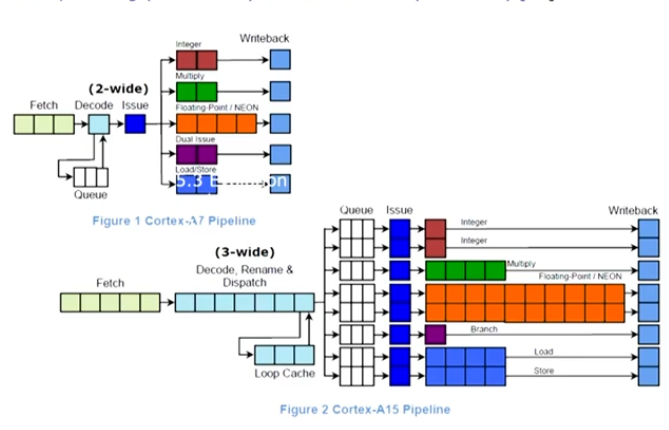
\includegraphics[width=0.8\textwidth]{biglittle}
    \centering
    \caption{big és LITTLE magok a Cortex-A7 processzorban}
    \label{fig:biglittle}
\end{figure}
Egy egyszerű big.LITTLE rendszer tartalmaz két big és két LITTLE magot (A15 és A7), amiket egy cache koherens hálózat köt össze (Cache Coherent Interconnect - CCI-400).
Alapesetben a LITTLE mag működik, ha nő a teljesítmény igény, átkapcsol a big magokra.

\subsection{Cortex-A processzorok teljesítmény növekedése}
Az ARM processzorok hatékonysága 2007-től 2016-ig a duplájára nőtt (IPC alapján).
A tényleges teljesítmény ugyanezen az időtávon 5-szörösére emelkedett, a fogyasztás pedig mindeközben a felére csökkent.

Az Intel processzorok ezalatt viszont kisebb hatékonyság növekedést értek el.

\subsection{Az ARM Cortex-A processzorok elterjedése}
Az ARM Cortex-A8 és A9 processzorok jelentek meg először széleskörben a mobil eszközöknél.

\section{A Cortex-A profilú CPU-k fejlődése (v8.2)}
Az ARMv8.2 egy jelentős előrelépést jelentett az ARM processzor fejlődésében.
2017-ben jelentek meg először, a Cortex-A55 és A75 processzorokkal (egyidőben az AMD Zennel).
Az 5-ös a nagy hatékonyságú, a 7-es pedig a nagy teljesítményű modell.

A modellcsalád kiegészült a Cortex-X1 processzorral, ami egy nagyon nagy teljesítményű processzor.

\subsection{Különbségek az ARMv8-hoz képest}
\begin{itemize}
    \item a magok frontendje szélesedett
    \item a futószalagok száma növekedett
\end{itemize}

\subsection{Fejlesztési roadmap}
Az ARM 2017-ben egy fejlesztési roadmapet tett közzé, amikor bejelentették a Deimos és Hercules modelleket (később az A-77 és A-78 nevet kapták).
Ekkor az ARM szerint a processzoraik teljesítményben felül fogják múlni az Intelt.
\begin{figure}[H]
    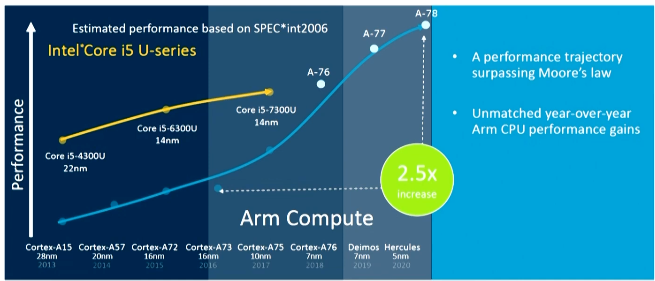
\includegraphics[width=0.8\textwidth]{armroad}
    \centering
    \caption{Az ARM által jósolt fejlődés}
    \label{fig:armroad}
\end{figure}

\subsection{A Cortex-X1 processzor}
A Cortex-X1 processzort 2020-ban jelentették be, a Cortex-A78-al közös alapokra épül.
Tervezése az Austin-i központban történt.
A bejelentése egy új program keretében történt, ez volt a Cortex-X Custom, ami a Built on ARM Cortex Technology evolúciója.
A program keretében lehetőség van a partnerrel közösen testreszabni a készülő processzorokat, mint pl. meghatározni a ROB méretét.
A készülő processzorok megtartják a Cortex nevet és az ARM márkát.

\subsubsection{Különbségek az A78-tól}
\begin{itemize}
    \item az A78 egy kiegyensúlyozott fejlesztés, az X1 viszont a teljesítményt helyezi előtérbe a fogyasztással szemben
    \item az A78 4 utasítású frontenddel szemben 5 utasításúval rendelkezik
    \item 2 helyett 4 SIMD futószalag van
    \item a cache-ek mérete is megnőtt
    \item a ROB méret is növekedett
\end{itemize}

\subsubsection{Eredmények}
A Cortex-X1-el nagyjából 20-30\%-os teljesítmény növekedést tudtak elérni.
\begin{figure}[H]
    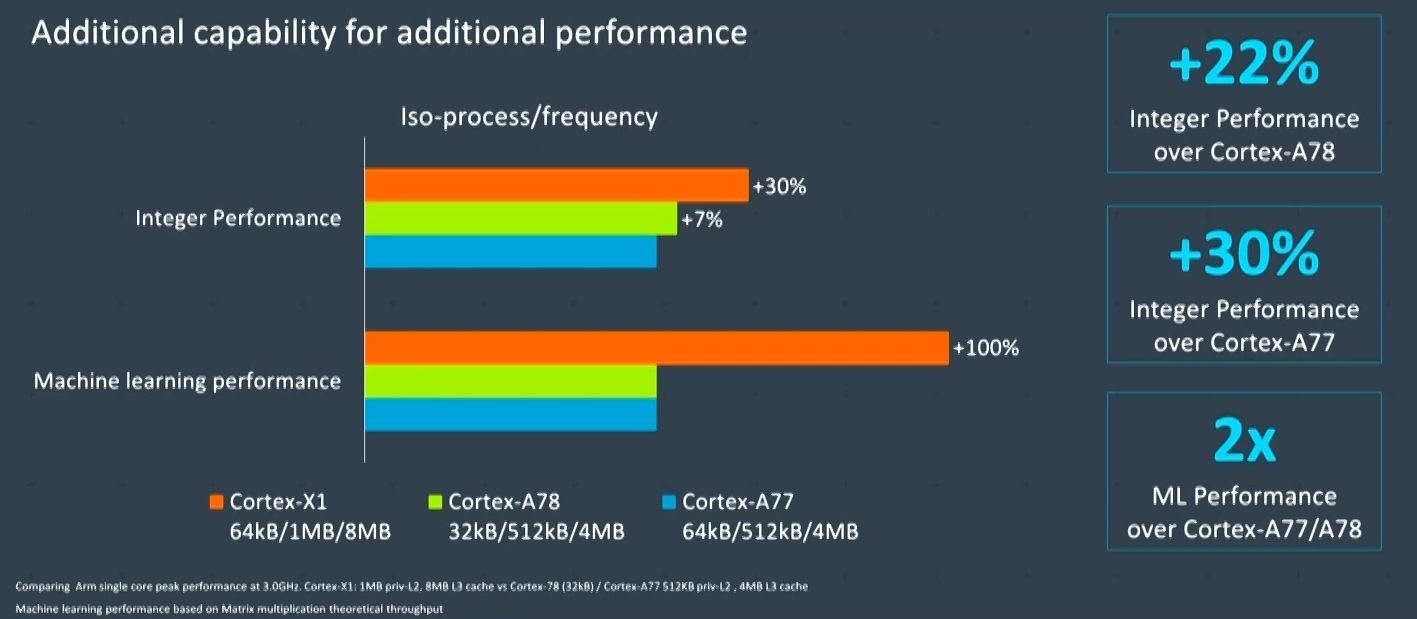
\includegraphics[width=0.8\textwidth]{perf}
    \centering
    \caption{Az ARM Cortex-X1 teljesítmény növekedése}
    \label{fig:perf}
\end{figure}

\section{Az ARMv9 ISA}
Az ARM 2021 márciusában jelentett be, az első processzorok 1-2 hónappal később jöttek ki.
Az első ilyen processzor a szerverekbe szánt Neoverse volt.

Az ARM célja az ARMv9-el a teljes felhasználási terület lefedése, a szenzoroktól a szerverekig.
Az ARM architektúra 9. verziója 10 évvel a 8-as után jelent meg.
Az új verzió visszafelé kompatibilis a korábbi architektúrákkal.

\subsection{Főbb fejlesztési területek}
\begin{itemize}
    \item vektor és digitális jelfeldolgozás (SVE2)
    \item mély tanulás
    \item többszálas programozás hatékonysága
    \item biztonság
\end{itemize}

\subsection{Vektor és digitális jelfeldolgozás (SVE2)}
Az ARM már korábban is támogatott vektoros kiterjesztéseket, ez volt az SVE (Scalable Vector Extension), ami az ARMv8.2 utasításkészlet egy opcionális kiterjesztése volt.
Ez főleg a tudományos alkalmazásokat támogatott, általános felhasználásra nem igazán volt alkalmas.

Ennek a hiányosságait küszöböli ki az SVE2, ami a teljes alkalmazói spektrumot lefedi és így a célja a Neon leváltása.

\subsubsection{Az SVE és SVE2 előnyei}
\begin{itemize}
    \item lehetővé tesznek változó hosszú, kvantált vektorméreteket
    \item lehetővé teszik a szóhossz független programozást - ennek segítségével a programozó ugyanazokat az utasításokat tudja használni a vektorhossztól függetlenül. Ezt predikátum regiszterekkel éri el az architektúra, ahol a bitek kijelölik az aktív adatmezőket. Következmény, hogy a kód más végrehajtó egységen is futtatható.
\end{itemize}

\subsection{ML}
A gépi tanulást az élet minden területén használjuk, ennek egy lényeges eleme a neurális hálók használata.
Az ARMv9 ezért támogatja a félpontosságú lebegőpontos számformátumot és a Google által kifejlesztett BFloat típusokat.
Ezen kívül támogatja a skalárszorzat számításokat is.

\subsection{Többszálú programozás támogatása}
Többszálú programoknál fennálhatnak versenyhelyzetek (race condition), ezek megoldására két mechanizmus lehetséges:
\begin{itemize}
    \item lockok - az adott memóriaterülethez egyszerre csak egy szál férhet hozzá
    \item tranzakciós memória - a rendszer ellenőrzi és javítja a konfliktusokat, hasonlóan az elágazásbecslés visszalépéséhez
\end{itemize}
A tranzakciós memóriát már más gyártók korábban is használták, az ARM is bevezette a v9-el.

\subsection{Biztonság}
A biztonság növelése érdekében bevezették a megbízható számítási architektúrát és a memória jelzőbitek (memory tagging) használatát.

\section{Az ARMv9 mikroarchitektúra}
Az ARM 2011-ben vezette be a big.LITTLE architektúrákat, ami két magcsoportot tartalmazott, klaszterenként max. 4 maggal.
Ezt váltotta a v8.2-ben a DynamIQ dinamikus mag klaszter, ahol már max. 8 kis mag lehet egy klaszterben, valamint a magokat tetszőlegesen lehet kombinálni, azzal a megkötéssel, hogy max. 4 nagy mag lehet.
A big.LITTLE-el ellentétben a DynamIQ architektúrában már saját L2 cache-t kaptak a magok.

Egy DynamIQ klaszter két részből áll:
\begin{itemize}
    \item magok
    \item DSU - DynamIQ Shared Unit
\end{itemize}

\subsection{A DSU}
\begin{itemize}
    \item viszonylag nagy L3 cache-t tartalmaz
    \item a rendszerhez 2x128 bites vagy 1x256 bites buszon kapcsolódik
    \item a disszipációkezelés magonként történik
\end{itemize}

\subsection{A DynamIQ klaszter fejlődése}
Az ARMv9 processzoroknál fejlesztették a DynamIQ klasztert is, a következő változások történtek:
\begin{itemize}
    \item 3 magtípust lehet használni
    \item szeletelt L3 cache és egyéb DSU egységek
    \item memória címkézés (Memory Tagging Extension) támogatása
    \item szélesebb, skálázható csatlakoztatás a DSU-nál
\end{itemize}

Az új magtípusok:
\begin{itemize}
    \item nagy teljesítményű mag
    \item nagy hatékonyságú big mag
    \item nagy hatékonyságú LITTLE mag
\end{itemize}
Tehát megjelent egy még gyorsabb magtípus.
Ezzel az ARM több felhasználási területet akar lefedni, pl. a laptopokat.

A DSU egyik nagyon fontos újítása, hanem egy szeletelt megvalósítás jelenik a korábbi monolit felépítés helyett.
A szeleteket egy gyűrűs kapcsolat fogja össze, két darab egyirányú gyűrűvel.
Míg a monolitikus egység egy belépési ponttal rendelkezik, a szeletelt cache-nél a szeletek önálló életet élnek, minden szelet önállóan tud kommunikálni.
Ennek előnye, hogy a szeletek párhuzamosan tudnak működni, ami gyorsítja a teljesítményt.
További előny, hogy a szeletek kisebbek, így kisebb a hozzáférési idő.
Hátrány viszont, hogy ha a keresett adat egy távolabbi szeletben van, tovább tart az elérése.
A rendszer tehát NUCA (Non-Uniform Cache Architecture) felépítést használ.

A szeletelésen kívül megnövelték még az L3 cache méretét.

\subsection{Memory Tagging Extension}
A memória gyakran biztonsági problémák forrása.
Az ebből adódó sérülékenységek elkerülésére az MTE bevezet zárakat és kulcsokat.
A zárak hozzá vannak rendelve a memóriához, 16 byte-onként egy 4 bites zárat definiálnak.
A hozzáférés során a virtuális címekhez kulcsokat rendelnek.
A kulcs csak akkor férhet hozzá egy területhez, ha megegyezik a zárral.

A kulcsok megoldásához felhasználták, hogy az ARMv8-A nem használja a pointerek legfelső byte-ját, ezt használják a kulcsra.

\subsection{Hozzáférési szélesség növelése} 
Korábban 2x128 vagy 1x256 bitet használtak a busz interfészhez, a 9-es verzió viszont megnégyszerezi ezt a hozzáférési szélességet.

\section{ARMv9-A-t megvalósító processzorok}
A Cortex családban három v9-es processzor jelent meg: Cortex-A510, Cortex-A710 és Cortex-X2.
Az előző generációkhoz képest 10-30\%-os teljesítménynövekedést, 20-30\%-os hatékonyság növekedést és 2x gépi tanulási teljesítményt tudnak.

A legnagyobb teljesítményű ARMv9-es processzor az ARM Cortex X2.
Az ARM Cortex-A710 és az X2 egymagos processzor, az A510 pedig kétmagos.
Az ARMv9-A alapú magklaszterek ezeket az egységeket tudják felhasználni.